\part{離散時間化}
    \chapter{背景}
        信号処理や制御工学では実用上、ディジタル計算機で実現するために連続時間信号をAD変換して離散領域で演算した後、DA変換して連続系である制御対象に入力する。
        よって手を加える前の物理系に於いて入力と制御対象の間に0次ホールド回路と演算回路が挟まった形になる。
        さらに、積分はEuler法や双一次変換で近似され、微分前進/後退差分や中心差分で近似される。
        この部ではこれらの離散時間化によるスペクトルへの影響を述べる。
    \chapter{0次ホールド}
    \section{0次ホールド機構の周波数特性}
        \subsection{背景}
            信号処理や制御工学では実用上、ディジタル計算機で実現するために連続時間信号をAD変換して離散領域で演算した後、DA変換して連続系である制御対象に入力する。
            よって手を加える前の物理系に於いて入力と制御対象の間に0次ホールド回路と演算回路が挟まった形になる。
            技術書の中にはこれをステップ入力に対するラプラス変換の積分と時間遅れとして表してゲインや位相を考えているものもあるが、これは厳密には正しくない。
            なぜなら、0次ホールド回路に正弦波を入れた際、通過した信号は細かいステップの集まりであり、元の正弦波に近いものの、完全な正弦波ではないからである。
            「ゲイン」や「位相変化」を厳密に定義できない。
            厳密には、Fourier変換してスペクトラムについて考える必要がある。
            とはいえ、無限に続く減衰しない信号のFourier変換は通常の関数の意味では存在しないし(超関数になる)、現実の測定器は窓関数で時間制限した信号のFourier変換を近似的に計算している。
            そこで本記事では窓関数付きのFourier変換の結果ついて考察する。
        \subsection{導出}
            \newcommand{\xd}{x_\text{d}}
            \newcommand{\Xd}{X_\text{d}}
            $f_0>0$とし、連続時間の複素正弦波信号$x:t\in\realNumbers\mapsto\exp(i 2\pi f_0 t)$を考える。
            サンプリング周期を$\Tsamp>0$とする。
            この周期で$x$を0次ホールドした信号を$\xd:t\in\realNumbers\mapsto x(\floor{t/\Tsamp}\Tsamp)$とする。
            次の図は$x$と$\xd$の実部を示したものである。
            \begin{figure}[H]
                \centering
                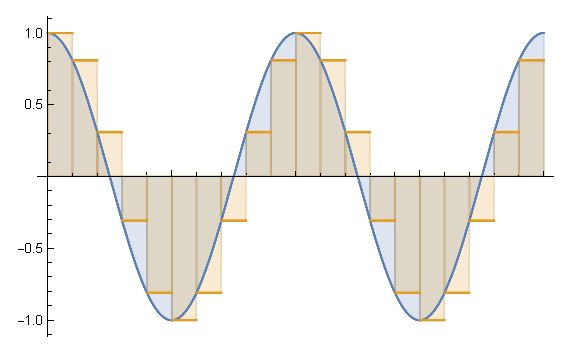
\includegraphics[keepaspectratio, scale=0.6]
                {\currfiledir/0-order-held-sinusoid.eps}
                \caption{元の信号とその0次ホールド}
            \end{figure}
            上の図より、$\xd$の基本周波数成分(周波数成分に於ける$f_0$に対応する成分)が$x$のそれより遅れることが予想される。
            このことを矩形窓を通した、周波数表示されたFourier変換で考察する。
            $N\in\naturalNumbers$とし、窓の幅を$T=N\Tsamp$とする。
            窓の幅を$\Tsamp$の整数倍に選んでいるが、非整数倍の場合でも幅を十分に大きくとれば小数部分に対応する区間の積分の$1/T$倍は無視できるほど小さくなり、最も近い整数倍の幅を用いた結果と殆ど一致する。
            $x$の窓付きFourier変換を窓の幅で規格化したものは次式である。
            \[ X(f) = \frac{1}{T} \integrate{0}{T}{x(t)\exp(-i 2\pi f t)}{}{t} = \frac{1}{i 2\pi(f-f_0)T}\left(1-\exp\left(-i 2\pi(f-f_0)T\right)\right) \]
            $\xd$の窓付きFourier変換は次式である。
            \begin{align*}
                \Xd(f) &= \frac{1}{T}\integrate{0}{T}{\xd(t)\exp(-i 2\pi f t)}{}{t} = \frac{1}{T}\sum_{k=0}^{N-1}\integrate{k\Tsamp}{(k+1)\Tsamp}{\xd(t)\exp(-i 2\pi f t)}{}{t} \\
                &= \frac{1}{T}\sum_{k=0}^{N-1}\exp(i 2\pi f_0 k\Tsamp)\integrate{k\Tsamp}{(k+1)\Tsamp}{\exp(-i 2\pi f t)}{}{t} \\
                &= \frac{1}{T}\sum_{k=0}^{N-1}\exp(i 2\pi f_0 k\Tsamp)\frac{1}{i 2\pi f}\exp(-i 2\pi f k\Tsamp)\left(1-\exp(-i 2\pi f \Tsamp)\right) \\
                &= \frac{1-\exp(-i 2\pi f\Tsamp)}{i 2\pi f}\frac{1}{T}\underbrace{\sum_{k=0}^{N-1}\exp(i 2\pi(f_0-f)k\Tsamp)}_{\text{(A)}} \\
                &= \frac{1-\exp(-i 2\pi f\Tsamp)}{i 2\pi f}\frac{1}{N\Tsamp}\exp(i\pi(f_0-f)(N-1)\Tsamp)\frac{\sin\pi(f-f_0)N\Tsamp}{\sin\pi(f-f_0)\Tsamp}
            \end{align*}
            最後の式を導くために、(A)に等比数列の和の公式を適用し、分母・分子それぞれ$\sin$が生じるように複素指数関数を括り出して整理した。
            \par
            $\xd$中の、周波数が$f_0$である成分の振幅と位相を調べる。
            $f\to f_0$の極限に関して次式が成り立つ。
            \[ \lim_{f\to f_0} \Xd(f) = \frac{1-\exp(-i 2\pi f_0\Tsamp)}{i 2\pi f_0\Tsamp} \]
            これより、上式に相当する振幅と位相の変化が生じる。
            サンプリングが十分に高速、すなわち$f_0\Tsamp\ll 1$であるとき上式は1に近づくので、振幅と位相の変化は無くなってゆく。
            \par
            次に、高調波領域を調べる。
            $|\Xd(f)|$は$1/\Tsamp$周期関数と$1/|f|$の積であるので、$|f|<\Tsamp/2$の部分の縮小コピーが高周波領域に於いて$1/\Tsamp$毎に現れる。
            これが高調波成分である。
        \subsection{数値例}
            今、$f_0=10,\;\Tsamp=10^{-2},\;N=200$とする。
            $f=f_0$に於ける振幅と位相は$|\Xd(f_0)| \approx 0.9836,\quad \angle \Xd(f_0) \approx \ang{-18.00}$となる。
            次の図は$f_0$近傍でのパワースペクトル$X,\Xd$を示したものである。
            \begin{figure}[H]
                \centering
                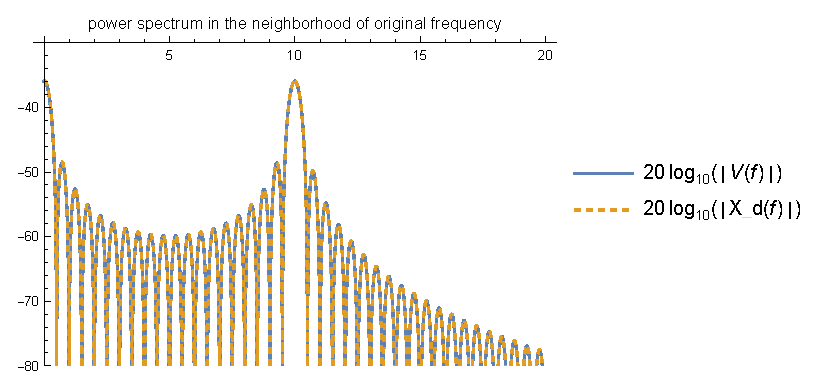
\includegraphics[keepaspectratio, scale=0.8]
                {\currfiledir/spectrum_in_the_neighborhood_of_original_frequency.eps}
                \caption{元の周波数の近傍でのパワースペクトル}
            \end{figure}
            低周波領域では両者が良く一致していることがわかる。
            \par
            次に高調波を見る。
            次の図はサンプリング周波数の3倍の範囲まで$X,\Xd$を示したものである。
            次の図は$x$と$\xd$の実部を示したものである。
            \begin{figure}[H]
                \centering
                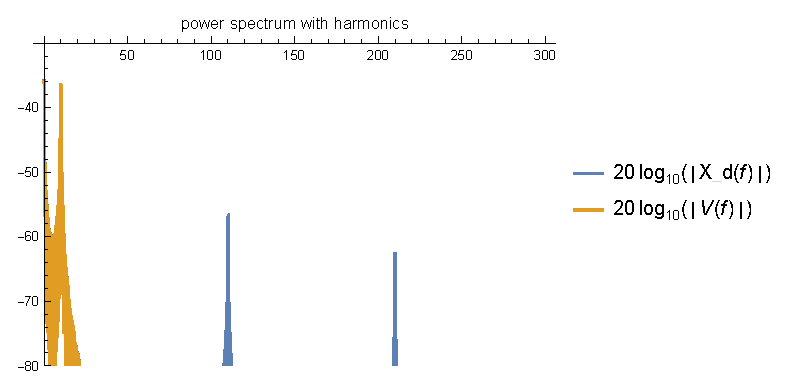
\includegraphics[keepaspectratio, scale=0.8]
                {\currfiledir/power_spectrum_with_harmonics.eps}
                \caption{高調波を含むパワースペクトル}
            \end{figure}
            この数値例を計算したMathematicaノートブックおよびMATLABスクリプトは下記のファイル名で保存されている。
            Gitリポジトリ内でファイル名検索すれば発見できるであろう。
            \begin{itemize}
                \item \href{\currfiledir/spectrum_of_zero-order-held-sine-wave.nb}{spectrum\_of\_zero\-order\-held\-sine\-wave.nb}
                \item \href{\currfiledir/spectrum_of_zero_order_held_sine_wave.m}{spectrum\_of\_zero\_order\_held\_sine\_wave.m}
            \end{itemize}
    \section{入力に0次ホールド機構を加えた連続時間システムのz変換}
        \subsection{背景}
            実用上、物理系をディジタル計算機で制御するために、連続系である制御対象と入力の間に「AD変換器」(0次ホールド回路+量子化器),「演算回路」,「DA変換器」(0次ホールド回路)が追加される。
            本節では、連続時間システムの入力に0次ホールド機構を追加したときのシステムの出力のうち、サンプリング時間の整数倍の時点に於いて出力が厳密に一致する離散時間システムのz変換を導出する。
        \subsection{導出}
            \newcommand{\ud}{u_\text{d}}
            \renewcommand{\uH}{u_\text{H}}
            \newcommand{\Ud}{U_\text{d}}
            元の連続時間システムのインパルス応答を$h:\realNumbers\to\complexNumbers$とし、そのラプラス変換を$H:\complexNumbers\to\complexNumbers$とする。
            この連続時間システムへの入力を$u:\realNumbers\to\complexNumbers$とする。
            但し$u(t)=0\;(t<0)$とする。
            サンプリング周期を$\Tsamp>0$とし、0次ホールドされた入力信号を$\ud:t\in\realNumbers\to u(\floor{t/\Tsamp}\Tsamp)$とする。
            Heavisideの単位ステップ関数を$\uH$とすると$\ud$は次式で表せる。
            \[ \ud(t) = \sum_{k=0}^\infty u(k\Tsamp)\left(\uH(t-k\Tsamp) - \uH(t-(k+1)\Tsamp)\right) \]
            これのラプラス変換を$U_\text{d}$とすると次式で表される。
            \[ \Ud(s) = \sum_{k=0}^\infty u(k\Tsamp)\frac{e^{-k\Tsamp s}}{s} \]

    \chapter{積分の離散近似}
    この部は文献\cite{digital-servo}に動機付けられて書いたものであり、その内容を再確認、深堀りしたもの、また派生して考えたことを記している。
    \section{Euler法}
        \subsection{背景}
            物理系をディジタル計算機で制御するにあたり、積分をEuler法で近似することがある。
            本節では正弦波をEuler法で近似的に積分した際の出力の窓関数付きFourier変換を導出し、高周波領域での位相変化、エイリアシングについて考察する。
        \subsection{導出}
            \newcommand{\xdd}{x_\text{dd}}
            $f_0>0$とし、連続時間の複素正弦波信号$u:t\in\realNumbers\mapsto\exp(i 2\pi f_0 t)$を考える。
            これを時刻$0$から$t\geq 0$まで積分した信号は$v(t) = \bigl(\exp(i 2\pi f_0 t)-1\bigr) / (i 2\pi f_0)$である。
            \ref{0次ホールドされた正弦波の周波数特性}と同様に、矩形窓を通した、周波数表示された$v$のFourier変換を考える(窓の幅をサンプリング周期の整数倍に限っても影響が少ないことの説明は\ref{0次ホールドされた正弦波の周波数特性}で述べられている)。
            $N\in\naturalNumbers$とし、窓の幅を$T=N\Ts$とする。
            $v$の窓付きFourier変換を窓の幅で規格化したものは次式である。
            但し計算は容易なので過程は省略した。
            \begin{align*}
                &\phantom{=} V(f) = \frac{1}{T} \integrate{0}{T}{v(t)\exp(-i 2\pi f t)}{}{t} \\
                &= \frac{1}{i 2\pi f_0 T} \left\{\frac{1}{i 2\pi (f-f_0)}\bigl[1 - \exp\bigl(-i 2\pi (f-f_0)T\bigr)\bigr] + \frac{1}{i 2\pi f}\bigl(\exp(-i 2\pi f T) - 1\bigr)\right\}
            \end{align*}
            次に、$u$の積分をサンプリング周期$\Ts>0$のEuler法で近似したものを考える。
            Euler法で積分した結果の離散時間信号を$\xdd:\integers\to\complexNumbers$とすると、これは漸化式$\xdd(n) = \xdd(n-1) + \Ts u\bigl((n-1)\Ts\bigr)$に従う。
            但し初期条件として$\xdd(0)=0$とする。
            この漸化式を解き、次式を得る。
            \[ \xdd(n) = \Ts\frac{1-\exp(i 2\pi f_0 n\Ts)}{1-\exp(i 2\pi f_0\Ts)} \]
            これを0次ホールドして得られる連続時間信号を$\xd(t) \coloneqq \xdd(\floor{t/\Ts}\Ts)$とする。
            先ほど$v$に対して行ったのと同様に窓付きFourier変換$\Xd$を計算すると、次式を得る。
            但し計算は容易なので過程の多くを省略した。
            \begin{align*}
                &\phantom{=} \Xd(f) = \frac{1}{T} \integrate{0}{T}{\xd(t)\exp(-i 2\pi f t)}{}{t} = \sum_{k=0}^{N-1} \frac{1}{T} \integrate{k\Ts}{(k+1)\Ts}{\xd(t)\exp(-i 2\pi f t)}{}{t} \\
                &= \frac{1}{i 2\pi f N}\times\frac{1-\exp(-i 2\pi f\Ts)}{1-\exp(i 2\pi f_0\Ts)} \left\{\frac{1-\exp(-i 2\pi f \Ts N)}{1-\exp(-i 2\pi f \Ts)} - \frac{1-\exp(-i 2\pi (f-f_0) \Ts N)}{1-\exp(-i 2\pi (f-f_0) \Ts)}\right\}
            \end{align*}
            $v$中の、周波数が$f_0$である成分の振幅と位相を調べる。
            $f\to f_0$の極限に関して次式が成り立つ。
            \[ \lim_{f\to f_0} V(f) = \frac{1}{i2\pi f_0}\left[1 + \frac{\exp(-i 2\pi f_0 T)-1}{i 2\pi f_0 T}\right] \]
            次に$\xd$中の、周波数が$f_0$である成分の振幅と位相を調べる。
            但し、$f_0\Ts < 1$と仮定する。
            次式が成り立つ。
            \[ \lim_{f\to f_0} \Xd(f) = \frac{1}{i 2\pi f_0 N}\times\frac{1-\exp(-i 2\pi f_0\Ts)}{1-\exp(i 2\pi f_0\Ts)}\left\{\frac{1-\exp(-i 2\pi f_0 \Ts N)}{1-\exp(-i 2\pi f_0 \Ts)} - N\right\} \]
            サンプリング周波数が十分高い、すなわち$f_0\Ts\ll 1$であるとき、次の近似式が成り立つ。
            \begin{align*}
                \lim_{f\to f_0} \Xd(f) &\approx \frac{1}{i 2\pi f_0 N}\times(-1)\left[\frac{1-\exp(-i 2\pi f_0 \Ts N)}{i 2\pi f_0 \Ts} - N\right] \\
                &= \frac{1}{i 2\pi f_0}\left[1 + \frac{\exp(-i 2\pi f_0 \Ts N)-1}{i 2\pi f_0 \Ts N}\right] = \frac{1}{i 2\pi f_0}\left[1 + \frac{\exp(-i 2\pi f_0 T)-1}{i 2\pi f_0 T}\right] \\
                &=  \lim_{f\to f_0} V(f)
            \end{align*}
        \subsection{数値例}
            今、$f_0=10,\;\Ts=10^{-2},\;N=200$とする。
            $f=f_0$に於ける$v$の振幅と位相の組は$(1/(20\pi),\;-\pi/2) \approx(1.59\times10^{-2},-1.57)$である。
            一方、$\xd$の振幅と位相の組はおよそ$(1.59\times10^{-2},-2.20)$である。
            \par
            次の図は$f_0$近傍でのエネルギー・スペクトラム密度$V,\Xd$を示したものである。
            \begin{figure}[H]
                \centering
                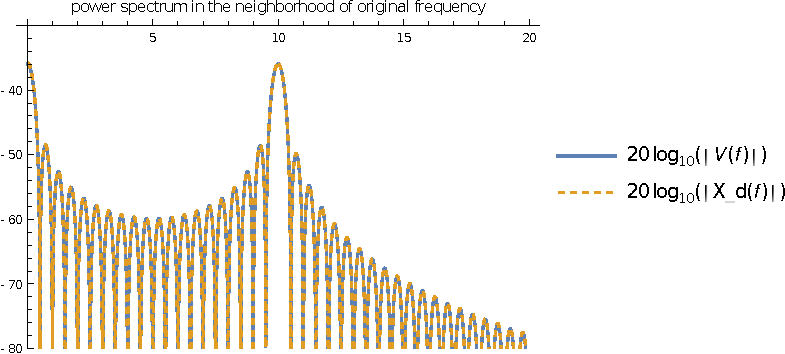
\includegraphics[keepaspectratio, scale=0.8]
                {\currfiledir/spectrum_in_the_neighborhood_of_original_frequency.pdf}
                \caption{元の周波数の近傍でのエネルギー・スペクトラム密度}
            \end{figure}
            低周波領域では絶対値が良く一致していることがわかる。
            \par
            次に高調波を見る。
            次の図はサンプリング周波数の3倍の範囲まで$V,\Xd$を示したものである。
            \begin{figure}[H]
                \centering
                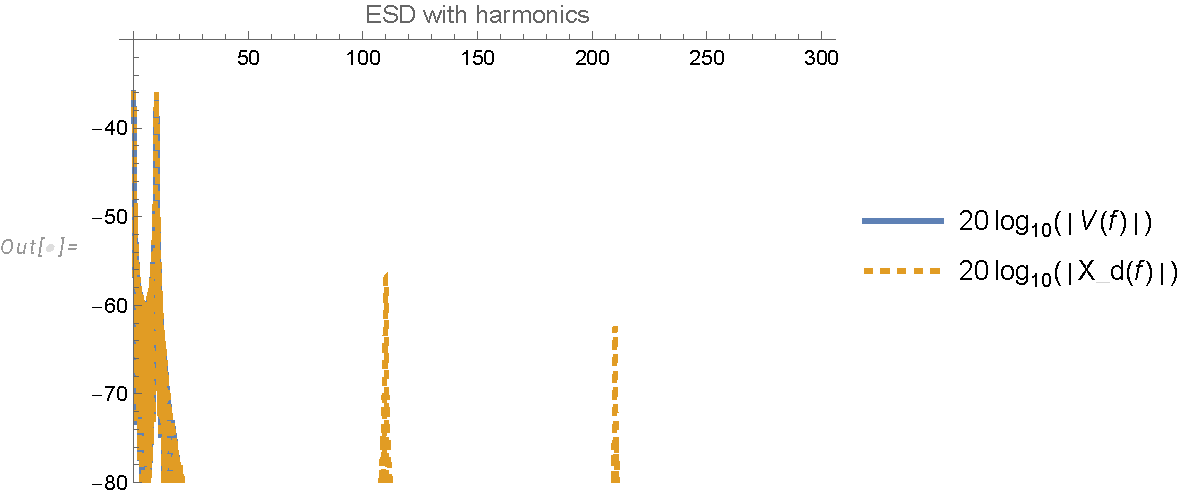
\includegraphics[keepaspectratio, scale=0.8]
                {\currfiledir/ESD_with_harmonics.pdf}
                \caption{高調波を含むエネルギー・スペクトラム密度}
            \end{figure}
            低周波の領域では$V,\Xd$が重なって判別できない。
            また、サンプリング周波数の整数倍の位置に高調波が生じていることが判る。
            \par
            この数値例を計算したMathematicaノートブックおよびMATLABスクリプトは下記のファイル名で保存されている。
            Gitリポジトリ内でファイル名検索すれば発見できるであろう。
            \begin{itemize}
                \item \href{\currfiledir/spectrum_of_integral-sine-wave_by_Euler-method.nb}{spectrum\_of\_integral\-sine-wave\_by\_Euler-method.nb}
                \item \href{\currfiledir/spectrum_of_integral_sine_wave_by_Euler_method.m}{spectrum\_of\_integral\_sine\_wave\_by\_Euler\_method.m}
            \end{itemize}

